% -*- TeX -*- -*- UK -*- -*- Soft -*-"

\chapter{Setting up WinEdt Projects}


\section{Setting up the Main File}

This section assumes that your project consists of more than one file (e.g. each chapter in a new file).  This technique requires one file as a root file, calling up all the other files.

Load the root file into the editor, and set it as the main file by using the menu path
$<$Project$>$$<$Set main file$>$.
This would set the current file as the root or main file for the project.  This is the file that will be compiled when the TeX or LaTeX buttons are pressed.

To ensure that the included file locations are saved as relative to the  main file, open the 
'Project Manager'  using the menu path $<$Project$>$$<$Project Manager$>$. Ensure that the relative file list check box is checked.  On previous version of WinEdt this relative check box appeared to be checked, but the relative search did not work. To fix this, first deselect the checkbox and 'OK' the dialog box, then reopen it again and select the relative file list check box.  This seemed to have fixed the problem in the past.

\centerline{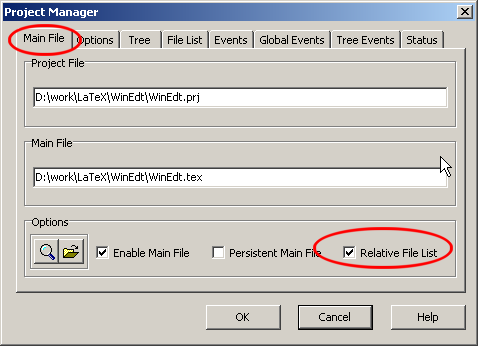
\includegraphics[bb= 0 0 512 387,scale=0.7]{eps/projectmanager.png}}









